\subsection{Compactness, Completeness, and Total Boundedness}\label{subsec:compactness-and-completeness}

% **Role:** abstract structure behind limits and continuity.
%
% Compactness, sequential compactness in metric spaces, Heine--Borel, completeness, total boundedness.


Compactness extracts finite or convergent structure from infinite behavior;\\
completeness asks whether Cauchy approximations converge internally.

\begin{definition} \label{def:open-cover-and-compactness} \hlt{Open Covers and Compact Sets}\\
Let $(X,d)$ be a metric space.
\begin{enumerate}[label=(\roman*)]
\setlength{\itemsep}{0pt}
\item A family $(G_\alpha)_{\alpha\in A}$ of open subsets of $X$ is an \hlt{open cover} of $E\subseteq X$ iff $E\subseteq\bigcup\limits_{\alpha\in A}G_\alpha$.
\item A set $K\subseteq X$ is \hlt{compact} iff every open cover of $K$ contains a finite subcover.
\end{enumerate}
\end{definition}

\begin{definition} \label{def:finite-intersection-property} \hlt{Finite Intersection Property}\\
Let $X$ be set, $\mathcal{F}\subseteq\mathcal{P}(X)$. Family $\mathcal{F}$ has \hlt{finite intersection property (FIP)} iff $(\forall\,\mathcal{F}_0\subseteq\mathcal{F})\,[0<|\mathcal{F}_0|<\infty\Rightarrow\bigcap\limits_{F\in\mathcal{F}_0}F\ne\emptyset]$.
\end{definition}

\begin{proposition} \label{prop:compactness-closed-fip-characterization} \hlt{Closed-Set Compactness Test}\\
A metric space $(X,d)$ is compact iff every nonempty family $\mathcal{F}$ of closed subsets of $X$ with FIP satisfies $\bigcap\limits_{F\in\mathcal{F}}F\ne\emptyset$.
\begin{proof}
\begin{enumerate}[label=\roman*.]
\setlength{\itemsep}{0pt}
\item[$(\Rightarrow)$] Assume $X$ is compact, and let $\emptyset\ne\mathcal{F}\subseteq\mathcal{P}(X)$ be a family of closed subsets with the finite intersection property.\\
If $X=\emptyset$, then $\mathcal{F}=\{\emptyset\}$, contrary to its finite intersection property. Suppose $X\ne\emptyset$ and $\bigcap\limits_{F\in\mathcal{F}}F=\emptyset$.\\
The family $\{X\setminus F:F\in\mathcal{F}\}$ is an open cover of $X$.\\
By compactness, choose $n\in\N$ and $F_1,\ldots,F_n\in\mathcal{F}$ such that $X=\bigcup\limits_{j=1}^{n}(X\setminus F_j)$.\\
Since $X\ne\emptyset$, $n\geq1$, whereas $\bigcap\limits_{j=1}^{n}F_j=\emptyset$. This contradicts the finite intersection property.
\item[$(\Leftarrow)$] Assume the closed-family condition, and let $(G_\alpha)_{\alpha\in A}$ be an open cover of $X$.\\
If $X=\emptyset$, the empty subfamily covers $X$. Suppose $X\ne\emptyset$ and no finite subcover exists.\\
Then $A\ne\emptyset$, and $\mathcal{F}\defeq\{X\setminus G_\alpha:\alpha\in A\}$ is a nonempty family of closed subsets. Let $\emptyset\ne\mathcal{F}_0\subseteq\mathcal{F}$ be finite.\\
For $C\in\mathcal{F}_0$, choose $\alpha_C\in A$ with $C=X\setminus G_{\alpha_C}$. Set $A_0\defeq\{\alpha_C:C\in\mathcal{F}_0\}$.\\
The finite set $A_0$ does not index a cover of $X$, so $\bigcap\limits_{C\in\mathcal{F}_0}C\ne\emptyset$. Thus $\mathcal{F}$ has the finite intersection property.\\
By the closed-family condition, $\bigcap\limits_{\alpha\in A}(X\setminus G_\alpha)\ne\emptyset$, contrary to $X\subseteq\bigcup\limits_{\alpha\in A}G_\alpha$.
\end{enumerate}
\hlt{Structural Commentary}: Taking complements exchanges finite subcovers with finite intersections.\\
\hlt{Key Insight}: An empty total intersection is already witnessed finitely.
\end{proof}
\end{proposition}

Figure \ref{fig:compactness-finite-subcover} depicts the finite extraction required by compactness.
\begin{illustrationfigure}[H]
  \centering
  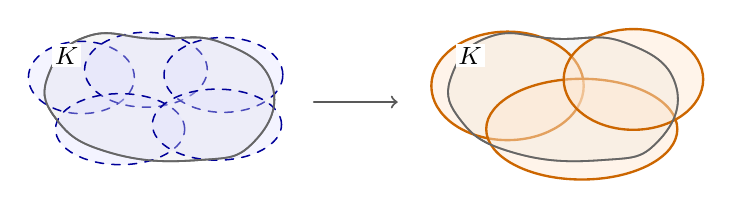
\begin{tikzpicture}[
  scale=0.82,
  every node/.style={font=\small},
  line cap=round,
  line join=round,
  compact/.style={draw=black!60, fill=gray!8, line width=0.65pt},
  compactoutline/.style={draw=black!60, line width=0.65pt},
  cover/.style={draw=blue!60!black, fill=blue!12, fill opacity=0.34, dashed, line width=0.55pt},
  chosen/.style={draw=orange!80!black, fill=orange!18, fill opacity=0.46, line width=0.85pt},
  arrow/.style={->, black!65, line width=0.75pt},
  note/.style={fill=white, inner sep=1pt}
]
  \begin{scope}
    \draw[compact]
      plot[smooth cycle, tension=0.8] coordinates {
        (-1.75,0.45) (-1.15,1.02) (-0.15,0.98) (0.92,0.92)
        (1.70,0.28) (1.42,-0.62) (0.55,-0.9) (-0.82,-0.78)
        (-1.65,-0.25)
      };
    \foreach \x/\y/\rx/\ry in {-1.25/0.38/0.82/0.56,-0.25/0.5/0.95/0.58,0.95/0.42/0.92/0.58,-0.65/-0.42/1.0/0.55,0.85/-0.35/1.0/0.55} {
      \draw[cover] (\x,\y) ellipse ({\rx} and {\ry});
    }
    \draw[compactoutline]
      plot[smooth cycle, tension=0.8] coordinates {
        (-1.75,0.45) (-1.15,1.02) (-0.15,0.98) (0.92,0.92)
        (1.70,0.28) (1.42,-0.62) (0.55,-0.9) (-0.82,-0.78)
        (-1.65,-0.25)
      };
    \node[note] at (-1.48,0.72) {$K$};
  \end{scope}

  \draw[arrow] (2.35,0) -- (3.65,0);

  \begin{scope}[xshift=6.25cm]
    \draw[compact]
      plot[smooth cycle, tension=0.8] coordinates {
        (-1.75,0.45) (-1.15,1.02) (-0.15,0.98) (0.92,0.92)
        (1.70,0.28) (1.42,-0.62) (0.55,-0.9) (-0.82,-0.78)
        (-1.65,-0.25)
      };
    \draw[chosen] (-0.9,0.25) ellipse (1.18 and 0.84);
    \draw[chosen] (0.25,-0.42) ellipse (1.48 and 0.78);
    \draw[chosen] (1.05,0.35) ellipse (1.08 and 0.78);
    \draw[compactoutline]
      plot[smooth cycle, tension=0.8] coordinates {
        (-1.75,0.45) (-1.15,1.02) (-0.15,0.98) (0.92,0.92)
        (1.70,0.28) (1.42,-0.62) (0.55,-0.9) (-0.82,-0.78)
        (-1.65,-0.25)
      };
    \node[note] at (-1.48,0.72) {$K$};
  \end{scope}
\end{tikzpicture}

  \caption{An arbitrary dashed cover of $K$ (left) is reduced to a finite solid subcover (right).}
  \label{fig:compactness-finite-subcover}
\end{illustrationfigure}

\begin{counterexample} \label{cex:open-interval-cover-without-finite-subcover} \hlt{An Open Cover Without a Finite Subcover}\\
For $x\in(0,1)$, set $O_x\defeq(\frac{x}{2},1)$. The family $(O_x)_{x\in(0,1)}$ covers $(0,1)$ because $(\forall\,y\in(0,1))\,y\in O_y$.\\
The empty subfamily does not cover $(0,1)$. Given $x_1,\ldots,x_n\in(0,1)$ with $n\geq1$, put $x'\defeq\min\limits_{1\leq i\leq n}x_i$.\\
Then $(\forall\,i\in\{1,\ldots,n\})\,O_{x_i}\subseteq O_{x'}$, while $(0,\frac{x'}{2}]\cap O_{x'}=\emptyset$. Hence no finite subfamily covers $(0,1)$.
\end{counterexample}

Figure \ref{fig:open-cover-no-finite-subcover} shows why the preceding cover of $(0,1)$ has no finite subcover.
\begin{illustrationfigure}[H]
  \centering
  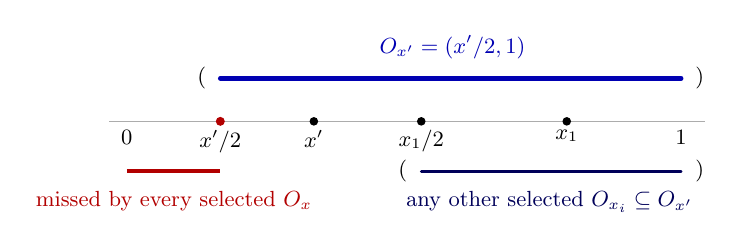
\begin{tikzpicture}[
  scale=0.88,
  transform shape,
  every node/.style={font=\small},
  axis/.style={gray!65, line width=0.55pt},
  cover/.style={blue!70!black, line width=1.7pt, line cap=round},
  subcover/.style={blue!35!black, line width=1.0pt, line cap=round},
  missed/.style={red!70!black, line width=1.35pt},
  point/.style={circle, fill=black, inner sep=1.25pt},
  missedpoint/.style={circle, fill=red!70!black, inner sep=1.3pt}
]
  \draw[axis] (-0.25,0) -- (8.35,0);
  \node[below] at (0,0) {$0$};
  \node[below] at (8,0) {$1$};

  \coordinate (xprimehalf) at (1.35,0);
  \coordinate (xprime) at (2.7,0);
  \coordinate (xonehalf) at (4.25,0);
  \coordinate (xone) at (6.35,0);

  \draw[missed] (0,-0.72) -- (1.35,-0.72);
  \node[red!70!black, below] at (0.68,-0.89) {missed by every selected $O_x$};

  \node[missedpoint] at (xprimehalf) {};
  \node[point] at (xprime) {};
  \node[point] at (xonehalf) {};
  \node[point] at (xone) {};

  \node[below] at (1.35,0) {$x'/2$};
  \node[below] at (2.7,0) {$x'$};
  \node[below] at (4.25,0) {$x_1/2$};
  \node[below] at (6.35,0) {$x_1$};

  \draw[cover] (1.35,0.62) -- (8,0.62);
  \node[anchor=east] at (1.27,0.62) {$($};
  \node[anchor=west] at (8.08,0.62) {$)$};
  \node[blue!70!black, above] at (4.7,0.78) {$O_{x'}=(x'/2,1)$};

  \draw[subcover] (4.25,-0.72) -- (8,-0.72);
  \node[anchor=east] at (4.17,-0.72) {$($};
  \node[anchor=west] at (8.08,-0.72) {$)$};
  \node[blue!35!black, below] at (6.1,-0.89) {any other selected $O_{x_i}\subseteq O_{x'}$};
\end{tikzpicture}

  \caption{For $x'=\min\limits_i x_i$, $(\forall\,i\in\{1,\ldots,n\})\,O_{x_i}\subseteq O_{x'}$, while $(0,\frac{x'}{2}]$ remains uncovered.}
  \label{fig:open-cover-no-finite-subcover}
\end{illustrationfigure}

\begin{theorem} \label{thm:compactness-independent-of-ambient-space} \hlt{Compactness Is Independent of the Ambient Space}\\
Let $(X,d)$ be a metric space, and suppose $K\subseteq Y\subseteq X$. Then $K$ is compact in $X$ iff it is compact in the subspace $(Y,d|_{Y\times Y})$.
\begin{proof}
\begin{enumerate}[label=\roman*.]
\setlength{\itemsep}{0pt}
\item[$(\Rightarrow)$] Let $(V_\alpha)_{\alpha\in A}$ be a subspace-open cover of $K$ in $Y$. Set $\mathcal{G}\defeq\{G\in\tau_d:(\exists\,\alpha\in A)\,Y\cap G=V_\alpha\}$.\\
The family $\mathcal{G}$ covers $K$ by Theorem \ref{thm:relative-open-intersection-with-open-set}. By compactness in $X$, choose a finite $\mathcal{G}_0\subseteq\mathcal{G}$ that covers $K$.\\
For $G\in\mathcal{G}_0$, choose $\alpha(G)\in A$ with $Y\cap G=V_{\alpha(G)}$. Since $K\subseteq Y$, the finite family $(V_{\alpha(G)})_{G\in\mathcal{G}_0}$ covers $K$.
\item[$(\Leftarrow)$] Let $(G_\alpha)_{\alpha\in A}$ be an open cover of $K$ in $X$. The family $(Y\cap G_\alpha)_{\alpha\in A}$ is a subspace-open cover of $K$ by Theorem \ref{thm:relative-open-intersection-with-open-set}.\\
By compactness in $Y$, some finite $F\subseteq A$ satisfies $K\subseteq\bigcup\limits_{\alpha\in F}(Y\cap G_\alpha)\subseteq\bigcup\limits_{\alpha\in F}G_\alpha$.
\end{enumerate}
\hlt{Structural Commentary}: Intersecting ambient opens with $Y$ transfers covers in both directions.\\
\hlt{Key Insight}: Finite subcovers survive restriction to the subspace.
\end{proof}
\end{theorem}

\begin{theorem} \label{thm:compact-subsets-of-metric-spaces-closed} \hlt{Compact Sets Are Closed}\\
Let $(X,d)$ be a metric space. Every compact set $K\subseteq X$ is closed in $X$.
\begin{proof}
\begin{enumerate}[label=(\roman*)]
\setlength{\itemsep}{0pt}
\item \hlt{Pointwise separation}: The claim holds for $K=\emptyset$ by Theorem \ref{thm:metric-open-closed-set-calculus}(iv). Suppose $K\ne\emptyset$, and fix $p\in X\setminus K$.\\
For $q\in K$, set $r_q\defeq\frac{1}{2}d(p,q)>0$, $V_q\defeq B_{r_q}(p)$, and $W_q\defeq B_{r_q}(q)$.\\
If $x\in V_q\cap W_q$, then $d(p,q)\leq d(p,x)+d(x,q)<2r_q=d(p,q)$, a contradiction. Thus $V_q\cap W_q=\emptyset$.
\item \hlt{Finite consolidation}: The family $(W_q)_{q\in K}$ covers $K$.\\
By compactness, choose $n\in\N$ and $q_1,\ldots,q_n\in K$ such that $K\subseteq\bigcup\limits_{i=1}^{n}W_{q_i}$.\\
The set $V\defeq\bigcap\limits_{i=1}^{n}V_{q_i}$ is open by Theorem \ref{thm:metric-open-closed-set-calculus}(iii), contains $p$, and is disjoint from $K$.
\item \hlt{Complement}: Thus $(\forall\,p\in X\setminus K)(\exists\,V\in\tau_d)\,p\in V\subseteq X\setminus K$. Hence $X\setminus K$ is open, so $K$ is closed.
\end{enumerate}
\hlt{Structural Commentary}: A finite cover converts pointwise disjoint balls into one complement neighborhood.\\
\hlt{Key Insight}: Half-distance balls around $p$ and $q$ cannot intersect.
\end{proof}
\end{theorem}

\begin{theorem} \label{thm:closed-subsets-of-compact-sets-compact} \hlt{Closed Subsets of Compact Sets Are Compact}\\
Let $(X,d)$ be a metric space, and suppose $F\subseteq K\subseteq X$. If $F$ is closed in $X$ and $K$ is compact, then $F$ is compact.
\begin{proof}
Let $(V_\alpha)_{\alpha\in A}$ be an open cover of $F$. Since $X\setminus F$ is open, $(V_\alpha)_{\alpha\in A}\cup\{X\setminus F\}$ covers $K$.\\
By compactness of $K$, some finite $F_0\subseteq A$ satisfies $K\subseteq(X\setminus F)\cup\bigcup\limits_{\alpha\in F_0}V_\alpha$. Therefore $F\subseteq\bigcup\limits_{\alpha\in F_0}V_\alpha$.\\
\hlt{Structural Commentary}: The open complement extends a cover of $F$ to one of $K$.\\
\hlt{Key Insight}: Discarding the complement leaves a finite cover of $F$.
\end{proof}
\end{theorem}

\begin{corollary} \label{cor:closed-intersection-compact} \hlt{Closed Intersections with Compact Sets}\\
Let $(X,d)$ be a metric space. If $F\subseteq X$ is closed and $K\subseteq X$ is compact, then $F\cap K$ is compact.
\begin{proof}
The set $K$ is closed by Theorem \ref{thm:compact-subsets-of-metric-spaces-closed}. Thus $F\cap K$ is closed by Theorem \ref{thm:metric-open-closed-set-calculus}(ii).\\
The set $F\cap K$ is compact by Theorem \ref{thm:closed-subsets-of-compact-sets-compact} with $F\cap K\subseteq K$.\\
\hlt{Structural Commentary}: Closed-set calculus makes $F\cap K$ closed; the closed-subset theorem transfers compactness.\\
\hlt{Key Insight}: The intersection remains a closed subset of compact $K$.
\end{proof}
\end{corollary}

\begin{theorem} \label{thm:compact-finite-intersection-property} \hlt{Finite Intersection Property for Compact Sets}\\
Let $(X,d)$ be a metric space, $(K_\alpha)_{\alpha\in A}$ be compact subsets of $X$,  $A\ne\emptyset$. If $(\forall\,F\subseteq A)\,[0<|F|<\infty\Rightarrow\bigcap\limits_{\alpha\in F}K_\alpha\ne\emptyset]$, then $\bigcap\limits_{\alpha\in A}K_\alpha\ne\emptyset$.
\begin{proof}
Choose $\alpha_0\in A$ and suppose $\bigcap\limits_{\alpha\in A}K_\alpha=\emptyset$. Then $K_{\alpha_0}\subseteq\bigcup\limits_{\alpha\in A}K_\alpha^c$. Each $K_\alpha^c$ is open by Theorem \ref{thm:compact-subsets-of-metric-spaces-closed}.\\
By compactness of $K_{\alpha_0}$, some finite $F\subseteq A$ satisfies $K_{\alpha_0}\subseteq\bigcup\limits_{\alpha\in F}K_\alpha^c$. Hence $\bigcap\limits_{\alpha\in F\cup\{\alpha_0\}}K_\alpha=\emptyset$, a contradiction.\\
\hlt{Structural Commentary}: Complements turn failure into a finite cover.\\
\hlt{Key Insight}: For compact sets, failure of intersection is already witnessed finitely.
\end{proof}
\end{theorem}

\begin{corollary} \label{cor:nested-nonempty-compact-intersection} \hlt{Nested Nonempty Compact Sets Intersect}\\
Let $(X,d)$ be a metric space. If $K_1\supseteq K_2\supseteq\cdots$ are nonempty compact subsets of $X$, then $\bigcap\limits_{n=1}^{\infty}K_n\ne\emptyset$.
\begin{proof}
Let $\emptyset\ne F\subseteq\N$ be finite, and put $m\defeq\max\limits_{n\in F}n$. Then $\bigcap\limits_{n\in F}K_n=K_m\ne\emptyset$ by nestedness.\\
Thus $(K_n)_{n\in\N}$ has the finite intersection property. Hence $\bigcap\limits_{n=1}^{\infty}K_n\ne\emptyset$ by Theorem \ref{thm:compact-finite-intersection-property}.\\
\hlt{Structural Commentary}: Nestedness reduces finite intersections to one term.\\
\hlt{Key Insight}: A nested compact sequence has the finite intersection property.
\end{proof}
\end{corollary}

\begin{theorem} \label{thm:infinite-subset-of-compact-has-limit-point} \hlt{Infinite Subsets of Compact Sets Have Limit Points}\\
Let $(X,d)$ be a metric space, let $K\subseteq X$ be compact, and let $E\subseteq K$ be infinite. Then $E^{\operatorname{acc}}\cap K\ne\emptyset$.
\begin{proof}
Suppose $E^{\operatorname{acc}}\cap K=\emptyset$, and set $\mathcal{U}\defeq\{B_r(q):q\in K,\ r>0,\ B_r(q)\cap(E\setminus\{q\})=\emptyset\}$.\\
The family $\mathcal{U}$ covers $K$ because no $q\in K$ is an accumulation point of $E$.\\
By compactness, choose $n\in\N$ and $B_{r_i}(q_i)\in\mathcal{U}$, $1\leq i\leq n$, such that $K\subseteq\bigcup\limits_{i=1}^{n}B_{r_i}(q_i)$.\\
Each selected ball meets $E$ in at most one point, so $|E|\leq n$, contrary to the infinitude of $E$.\\
\hlt{Structural Commentary}: Compactness reduces locally isolated intersections with $E$ to finitely many balls.\\
\hlt{Key Insight}: Finitely many one-point intersections cannot cover infinite $E$.
\end{proof}
\end{theorem}

\begin{definition} \label{def:sequentially-compact-metric-space} \hlt{Sequential Compactness}\\
A metric space $(X,d)$ is \hlt{sequentially compact} iff every sequence in $X$ has a subsequence converging in $X$.
\end{definition}

\begin{theorem} \label{thm:compact-sequential-subsequence} \hlt{Compactness Produces Convergent Subsequences}\\
If $(p_n)$ is a sequence in a compact metric space $(X,d)$, then some subsequence $(p_{n_i})$ converges to a point $p\in X$.
\begin{proof}
Let $E\defeq\{p_n:n\in\N\}$. If $E$ is finite and $(\forall\,q\in E)\,|\{n\in\N:p_n=q\}|<\infty$, then $\N$ is finite, a contradiction.\\
Thus some $p\in E$ occurs infinitely often when $E$ is finite, and $(\forall\,r>0)(\forall\,N\in\N)(\exists\,n\geq N)\,p_n\in B_r(p)$.\\
Suppose $E$ is infinite. Some $p\in E^{\operatorname{acc}}\cap X$ exists by Theorem \ref{thm:infinite-subset-of-compact-has-limit-point} with $K=X$.\\
Fix $r>0$ and $N\in\N$. The set $B_r(p)\cap E$ is infinite by Theorem \ref{thm:limit-point-neighborhoods-infinitely-many}, whereas $\{p_1,\ldots,p_{N-1}\}$ is finite.\\
Therefore $(\exists\,n\geq N)\,p_n\in B_r(p)$. In either case, a subsequence converges to $p$ by Proposition \ref{prop:sequence-limit-points-subsequential-limits}, $(i)\Rightarrow(ii)$.\\
\hlt{Structural Commentary}: Finite ranges repeat; infinite compact ranges contain an accumulation point.\\
\hlt{Key Insight}: Repetition and accumulation both create a convergent subsequence.
\end{proof}
\end{theorem}

\begin{definition} \label{def:cauchy-sequence} \hlt{Cauchy Sequence}\\
A sequence $(p_n)$ in a metric space $(X,d)$ is \hlt{Cauchy} if $(\forall\,\varepsilon>0)(\exists\,N\in\N)(\forall\,m,n\geq N)\, d(p_m,p_n)<\varepsilon$.
\end{definition}

\begin{definition} \label{def:diameter-of-metric-set} \hlt{Diameter}\\
Let $(X,d)$ be a metric space and $\emptyset\ne E\subseteq X$. The \hlt{diameter} of $E$ is $\diam E\defeq\sup\limits_{\overline{\R}}\{d(p,q):p,q\in E\}\in[0,+\infty]$.
\end{definition}

\begin{proposition} \label{prop:diameter-basic-properties} \hlt{Basic Diameter Properties}\\
Let $(X,d)$ be a metric space and let $\emptyset\ne E,F\subseteq X$.
\begin{enumerate}[label=(\roman*)]
\setlength{\itemsep}{0pt}
\item $E$ is bounded iff $\diam E<\infty$.
\item $\diam E=0\Longleftrightarrow |E|=1$.
\item $E\subseteq F\Longrightarrow\diam E\leq\diam F$.
\item $E,F$ bounded $\Longrightarrow E\cup F$ bounded.
\end{enumerate}
\begin{proof}
\begin{enumerate}[label=(\roman*)]
\setlength{\itemsep}{0pt}
\item[$(i)$] ($\Rightarrow$) If $E$ is bounded, choose $q\in X$ and $M>0$ such that $E\subseteq B_M(q)$.\\
Then $(\forall\,x,y\in E)\,d(x,y)<2M$ by the triangle inequality, so $\diam E\leq2M<\infty$.\\
\item[$(i)$] ($\Leftarrow$) If $\diam E<\infty$ and $q\in E$, then $E\subseteq B_{\diam E+1}(q)$, so $E$ is bounded.
\item[$(ii)$] ($\Rightarrow$) If $\diam E=0$, then $(\forall\,x,y\in E)\,d(x,y)=0$. Thus all points of the nonempty set $E$ are equal, and $|E|=1$.\\
\item[$(ii)$] ($\Leftarrow$) If $|E|=1$, then $(\forall\,x,y\in E)\,d(x,y)=0$, so $\diam E=0$.
\item[$(iii)$] Since $\{d(x,y):x,y\in E\}\subseteq\{d(x,y):x,y\in F\}$, $\diam E\leq\diam F$ by monotonicity of the supremum.
\item[$(iv)$] Choose $e\in E$, $f\in F$, and set $D\defeq\diam E+d(e,f)+\diam F<\infty$.\\
If $x,y$ lie in the same one of $E,F$, then $d(x,y)\leq D$. Otherwise, after swapping $x,y$, assume $x\in E$ and $y\in F$.\\
Then $d(x,y)\leq d(x,e)+d(e,f)+d(f,y)\leq D$. Thus $\diam(E\cup F)\leq D<\infty$, so $E\cup F$ is bounded by (i).
\end{enumerate}
\hlt{Structural Commentary}: Ball bounds control diameters; bridge points control cross-distances in unions.\\
\hlt{Key Insight}: One bridge distance joins two bounded sets.
\end{proof}
\end{proposition}

\begin{proposition} \label{prop:cauchy-tail-diameters} \hlt{Cauchy Sequences and Tail Diameters}\\
For $(p_n)$ in a metric space $X$, set $E_N\defeq\{p_j:j\geq N\}$. Then $(p_n)$ is Cauchy if and only if $\diam E_N\to0$.
\begin{proof}
\begin{enumerate}[label=\roman*.]
\setlength{\itemsep}{0pt}
\item[$(\Rightarrow)$] Given $\varepsilon>0$, choose $N_0$ so that $m,n\geq N_0$ implies $d(p_m,p_n)<\frac{\varepsilon}{2}$.\\
If $N\geq N_0$, then $(\forall\,m,n\geq N)\,d(p_m,p_n)<\frac{\varepsilon}{2}$, so $\diam E_N\leq\frac{\varepsilon}{2}<\varepsilon$.
\item[$(\Leftarrow)$] Given $\varepsilon>0$, choose $N_0$ with $\diam E_{N_0}<\varepsilon$. If $m,n\geq N_0$, then $p_m,p_n\in E_{N_0}$, hence $d(p_m,p_n)\leq\diam E_{N_0}<\varepsilon$.
\end{enumerate}
\hlt{Structural Commentary}: The Cauchy quantifiers match convergence of the decreasing tail diameters.\\
\hlt{Key Insight}: Tail diameter measures mutual closeness without naming a limit.
\end{proof}
\end{proposition}

\begin{definition} \label{def:contracting-sequence-of-metric-sets} \hlt{Contracting Sequence of Sets}\\
Let $(X,d)$ be a metric space and let $(F_n)_{n\geq1}$ satisfy $\emptyset\ne F_n\subseteq X$.
\begin{enumerate}[label=(\roman*)]
\setlength{\itemsep}{0pt}
\item The sequence $(F_n)$ is \hlt{descending} iff $(\forall\,n\geq1)\,F_{n+1}\subseteq F_n$.
\item The sequence $(F_n)$ is \hlt{contracting} iff it is descending and $\diam F_n\to0$.
\end{enumerate}
\end{definition}

Figure \ref{fig:cauchy-tail-diameters} visualizes the tail-diameter criterion for Cauchy sequences.
\begin{illustrationfigure}[H]
  \centering
  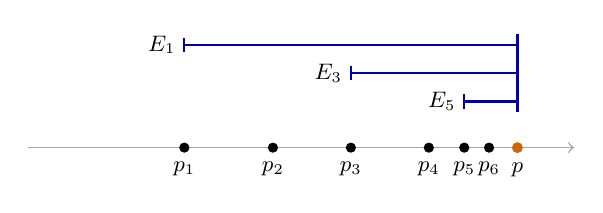
\begin{tikzpicture}[
  scale=0.90,
  transform shape,
  every node/.style={font=\small},
  axis/.style={->, gray!70, line width=0.55pt},
  tail/.style={blue!70!black, line width=0.8pt},
  dot/.style={circle, fill=black, inner sep=1.45pt},
  limit/.style={circle, fill=orange!80!black, inner sep=1.55pt}
]
  \draw[axis] (-0.2,0) -- (7.5,0);
  \node[limit,label=below:$p$] at (6.7,0) {};

  \foreach \x/\lab in {2.0/p_1,3.25/p_2,4.35/p_3,5.45/p_4,5.95/p_5,6.30/p_6} {
    \node[dot,label=below:\(\lab\)] at (\x,0) {};
  }

  \draw[tail] (2.0,1.45) -- (6.7,1.45);
  \draw[tail] (4.35,1.05) -- (6.7,1.05);
  \draw[tail] (5.95,0.65) -- (6.7,0.65);

  \node[left] at (2.0,1.45) {$\diam E_1$};
  \node[left] at (4.35,1.05) {$\diam E_3$};
  \node[left] at (5.95,0.65) {$\diam E_5$};

  \draw[tail] (2.0,1.35) -- (2.0,1.55);
  \draw[tail] (4.35,0.95) -- (4.35,1.15);
  \draw[tail] (5.95,0.55) -- (5.95,0.75);
  \draw[tail] (6.7,0.5) -- (6.7,1.6);
\end{tikzpicture}

  \caption{Tail diameters $\diam E_N$ shrink toward $0$.}
  \label{fig:cauchy-tail-diameters}
\end{illustrationfigure}

\begin{theorem} \label{thm:nested-compact-diameters-singleton} \hlt{Nested Compact Sets with Shrinking Diameter}\\
Let $(X,d)$ be a metric space.
\begin{enumerate}[label=(\roman*)]
\setlength{\itemsep}{0pt}
\item If $\emptyset\ne E\subseteq X$, then $\diam\overline{E}=\diam E$.
\item If $K_1\supseteq K_2\supseteq\cdots$ are nonempty compact subsets of $X$ and $\diam K_n\to0$, then $\left|\bigcap\limits_{n=1}^{\infty}K_n\right|=1$.
\end{enumerate}
\begin{proof}
\begin{enumerate}[label=(\roman*)]
\setlength{\itemsep}{0pt}
\item Since $E\subseteq\overline{E}$, $\diam E\leq\diam\overline{E}$ by Proposition \ref{prop:diameter-basic-properties}(iii). If $\diam E=+\infty$, equality follows.\\
Suppose $\diam E<\infty$. For $p,q\in\overline{E}$ and $\varepsilon>0$, choose $p',q'\in E$ with $d(p,p'),d(q,q')<\frac{\varepsilon}{2}$.\\
Then $d(p,q)<\diam E+\varepsilon$. Since $\varepsilon>0$ is arbitrary, $d(p,q)\leq\diam E$; hence $\diam\overline{E}\leq\diam E$.
\item Set $I\defeq\bigcap\limits_{n=1}^{\infty}K_n$. Then $I\ne\emptyset$ by Corollary \ref{cor:nested-nonempty-compact-intersection}.\\
For $x,y\in I$, $(\forall\,n\in\N)\,d(x,y)\leq\diam K_n$, so $d(x,y)=0$ by $\diam K_n\to0$. Thus $x=y$, and $|I|=1$.
\end{enumerate}
\hlt{Structural Commentary}: Closure preserves diameter; nested compactness and shrinking diameters split existence from uniqueness.\\
\hlt{Key Insight}: Every two intersection points have distance zero.
\end{proof}
\end{theorem}

\begin{theorem} \label{thm:cauchy-convergence-criterion} \hlt{Cauchy Criterion and Completeness Results}
\begin{enumerate}[label=(\roman*)]
\setlength{\itemsep}{0pt}
\item Every convergent sequence in a metric space is Cauchy.
\item Every Cauchy sequence in a compact metric space $X$ converges in $X$.
\end{enumerate}
\begin{proof}
\begin{enumerate}[label=(\roman*)]
\setlength{\itemsep}{0pt}
\item If $p_n\to p$, then for $\varepsilon>0$ choose $N$ with $d(p_n,p)<\frac{\varepsilon}{2}$ for $n\geq N$. For $m,n\geq N$, $d(p_m,p_n)\leq d(p_m,p)+d(p,p_n)<\varepsilon$.
\item Let $(p_n)$ be Cauchy in compact $X$, and set $E_N\defeq\{p_j:j\geq N\}$ and $F_N\defeq\overline{E_N}$. Each $F_N$ is nonempty.\\
Since $E_{N+1}\subseteq E_N\subseteq F_N$, one has $F_{N+1}\subseteq F_N$ by Theorem \ref{thm:closure-smallest-closed-containing-set}(iii).\\
Each $F_N$ is closed by Theorem \ref{thm:closure-smallest-closed-containing-set}(i), hence compact by Theorem \ref{thm:closed-subsets-of-compact-sets-compact}.\\
The convergence $\diam F_N=\diam E_N\to0$ holds by Proposition \ref{prop:cauchy-tail-diameters} and Theorem \ref{thm:nested-compact-diameters-singleton}(i).\\
The relation $(\exists\,p\in X)\,\bigcap\limits_{N=1}^{\infty}F_N=\{p\}$ holds by Theorem \ref{thm:nested-compact-diameters-singleton}(ii).\\
Given $\varepsilon>0$, choose $N$ with $\diam F_N<\varepsilon$. For $n\geq N$, both $p_n,p\in F_N$, so $d(p_n,p)<\varepsilon$.
\end{enumerate}
\hlt{Structural Commentary}: Cauchy tails create a contracting nest whose compact intersection supplies the limit.\\
\hlt{Key Insight}: Shrinking closed tails trap every late term near one point.
\end{proof}
\end{theorem}

\begin{lemma} \label{lem:cauchy-sequence-with-convergent-subsequence} \hlt{A Cauchy Sequence with a Convergent Subsequence Converges}\\
Let $(p_n)$ be a Cauchy sequence in a metric space $X$. If some subsequence $(p_{n_j})$ converges to $p\in X$, then $p_n\to p$.
\begin{proof}
Given $\varepsilon>0$, choose $N_0$ so that $m,n\geq N_0$ implies $d(p_m,p_n)<\frac{\varepsilon}{2}$.\\
Choose $j\geq N_0$ with $d(p_{n_j},p)<\frac{\varepsilon}{2}$; then $n_j\geq j\geq N_0$. For $n\geq N_0$, $d(p_n,p)\leq d(p_n,p_{n_j})+d(p_{n_j},p)<\varepsilon$.\\
\hlt{Structural Commentary}: A late subsequence term links the Cauchy tail to the subsequential limit.\\
\hlt{Key Insight}: One convergent thread fixes the destination of the entire tail.
\end{proof}
\end{lemma}

\begin{proposition} \label{prop:cauchy-sequences-bounded-distance-converges} \hlt{Boundedness and Distances of Cauchy Sequences}\\
Let $(X,d)$ be a metric space.
\begin{enumerate}[label=(\roman*)]
\setlength{\itemsep}{0pt}
\item If $(p_n)$ is Cauchy, then $\operatorname{ran}(p_n)$ is bounded.
\item If $(p_n)$ and $(q_n)$ are Cauchy, then $(d(p_n,q_n))$ converges in $\R$.
\item A bounded real sequence need not be Cauchy.
\end{enumerate}
\begin{proof}
\begin{enumerate}[label=(\roman*)]
\setlength{\itemsep}{0pt}
\item Choose $N\in\N$ with $m,n\geq N\Longrightarrow d(p_m,p_n)<1$, and set $R\defeq1+\max\limits_{1\leq j\leq N}d(p_j,p_N)$.\\
If $n\leq N$, then $d(p_n,p_N)<R$; if $n\geq N$, then $d(p_n,p_N)<1\leq R$. Hence $\operatorname{ran}(p_n)\subseteq B_R(p_N)$.
\item Let $(p_n)$, $(q_n)$ be Cauchy. For $m,n\in\N$, by triangle inequality, $|d(p_n,q_n)-d(p_m,q_m)|\leq d(p_n,p_m)+d(q_n,q_m)$.\\
Given $\varepsilon>0$, both terms on the right are less than $\frac{\varepsilon}{2}$ for sufficiently large $m,n$.\\
Hence $(d(p_n,q_n))$ is Cauchy in $\R$ and converges by Theorem \ref{thm:real-cauchy-convergence-criterion}.
\item Let $a_n\defeq(-1)^n$. Then $(\forall\,n\in\N)\,|a_n|\leq1$, so $(a_n)$ is bounded.\\
For $N\in\N$, choose even $m\geq N$ and odd $n\geq N$; then $|a_m-a_n|=2$. Thus $(a_n)$ is not Cauchy.
\end{enumerate}
\hlt{Structural Commentary}: A bounded tail controls the range; the four-point estimate controls pairwise distances.\\
\hlt{Key Insight}: Cauchy control persists under the metric map.
\end{proof}
\end{proposition}

\begin{definition} \label{def:complete-metric-space} \hlt{Complete Metric Space}\\
A metric space $(X,d)$ is \hlt{complete} iff every Cauchy sequence in $X$ converges in $X$.
\end{definition}

\begin{corollary} \label{cor:compact-metric-spaces-complete} \hlt{Compact Metric Spaces Are Complete}\\
Every compact metric space is complete.
\begin{proof}
Every Cauchy sequence converges to a point of the space by Theorem \ref{thm:cauchy-convergence-criterion}(ii); hence the space is complete.\\
\hlt{Structural Commentary}: The compact Cauchy criterion discharges the defining convergence requirement.\\
\hlt{Key Insight}: Compactness keeps every Cauchy limit inside the space.
\end{proof}
\end{corollary}

\begin{remark} \label{rem:boundedness-and-intrinsic-metric-properties} \hlt{Intrinsic and Ambient Metric Properties}\\
For $E\subseteq X$ in a metric space $(X,d)$, boundedness, compactness, and completeness are intrinsic to $d|_{E\times E}$.\\
In contrast, openness, closedness, and perfection depend on the ambient metric space.
\end{remark}

\begin{proposition} \label{prop:basic-completeness-consequences} \hlt{Completeness and Closed Subspaces}\\
Let $(X,d)$ be a metric space, let $E\subseteq X$, and set $d_E\defeq d|_{E\times E}$.
\begin{enumerate}[label=(\roman*)]
\setlength{\itemsep}{0pt}
\item If $(E,d_E)$ is complete, then $E$ is closed in $X$, equivalently $E=\overline{E}^{\,X}$.
\item If $(X,d)$ is complete, then $(E,d_E)$ is complete if and only if $E$ is closed in $X$, equivalently $E=\overline{E}^{\,X}$.
\end{enumerate}
\begin{proof}
\begin{enumerate}[label=(\roman*)]
\setlength{\itemsep}{0pt}
\item[$(i)$] Assume $(E,d_E)$ is complete, and let $(p_n)$ be a sequence in $E$ with $p_n\to p\in X$.\\
The sequence is Cauchy in $X$ by Theorem \ref{thm:cauchy-convergence-criterion}(i), hence it is Cauchy in $(E,d_E)$.\\
Choose $q\in E$ with $p_n\to q$ in $(E,d_E)$ by completeness. The same convergence holds in $X$ because $d_E=d|_{E\times E}$.\\
Equality $p=q$ holds by Theorem \ref{thm:metric-sequence-basic-properties}(ii); $E$ is closed by Theorem \ref{thm:closed-sets-and-limit-points-via-sequences}(ii). Equality $E=\overline{E}^{\,X}$ holds by Theorem \ref{thm:closure-smallest-closed-containing-set}(ii).
\item[$(ii)$] ($\Rightarrow$) Assume $(X,d)$ and $(E,d_E)$ are complete. Then $E=\overline{E}^{\,X}$ by (i).
\item[$(ii)$] ($\Leftarrow$) Assume $(X,d)$ is complete and $E=\overline{E}^{\,X}$. Then $E$ is closed by Theorem \ref{thm:closure-smallest-closed-containing-set}(ii).\\
If $(p_n)$ is Cauchy in $(E,d_E)$, then it is Cauchy in $X$, and $p_n\to p\in X$ by completeness.\\
The membership $p\in E$ holds by Theorem \ref{thm:closed-sets-and-limit-points-via-sequences}(ii). Thus every Cauchy sequence in $(E,d_E)$ converges in $(E,d_E)$.
\end{enumerate}
\hlt{Structural Commentary}: Subspace completeness forces closure; ambient completeness plus closure returns subspace limits.\\
\hlt{Key Insight}: Closedness is exactly the limit-retention condition.
\end{proof}
\end{proposition}

\begin{theorem} \label{thm:cantor-intersection-complete-metric-space} \hlt{Cantor Intersection Theorem}\\
Let $(X,d)$ be a metric space. Then $X$ is complete iff every contracting sequence $(F_n)_{n\geq1}$ of closed subsets of $X$ satisfies $\left|\bigcap\limits_{n=1}^{\infty}F_n\right|=1$.
\begin{proof}
\begin{enumerate}[label=\roman*.]
\setlength{\itemsep}{0pt}
\item[$(\Rightarrow)$] Assume $X$ is complete, and let $(F_n)$ satisfy the stated hypotheses. Choose $(x_n)$ with $(\forall\,n\in\N)\,x_n\in F_n$.\\
Given $\varepsilon>0$, choose $N$ with $\diam F_N<\varepsilon$. For $m,n\geq N$, descendingness places $x_m,x_n$ in $F_N$, so $d(x_m,x_n)<\varepsilon$.\\
The sequence $(x_n)$ is Cauchy, and $x_n\to x\in X$ by completeness.\\
For $N\in\N$, the tail $(x_n)_{n\geq N}$ lies in closed $F_N$, so $x\in F_N$ by Theorem \ref{thm:closed-sets-and-limit-points-via-sequences}(ii).\\
Hence $x\in\bigcap\limits_{N=1}^{\infty}F_N$. If $y\in\bigcap\limits_{N=1}^{\infty}F_N$, then $(\forall\,N\in\N)\,d(x,y)\leq\diam F_N$, so $x=y$ by $\diam F_N\to0$.
\item[$(\Leftarrow)$] Assume the intersection property, and let $(x_n)$ be Cauchy. Set $E_N\defeq\{x_n:n\geq N\}$ and $F_N\defeq\overline{E_N}$ for $N\in\N$.\\
Each $F_N$ is nonempty and closed by Theorem \ref{thm:closure-smallest-closed-containing-set}(i).\\
The inclusions $E_{N+1}\subseteq E_N\subseteq F_N$ imply $F_{N+1}\subseteq F_N$ by Theorem \ref{thm:closure-smallest-closed-containing-set}(iii).\\
The convergence $\diam F_N=\diam E_N\to0$ holds by Proposition \ref{prop:cauchy-tail-diameters} and Theorem \ref{thm:nested-compact-diameters-singleton}(i).\\
Choose $x\in X$ with $\bigcap\limits_{N=1}^{\infty}F_N=\{x\}$ by the intersection property.\\
Given $\varepsilon>0$, choose $N$ with $\diam F_N<\varepsilon$. If $n\geq N$, then $x_n,x\in F_N$, so $d(x_n,x)<\varepsilon$. Thus $x_n\to x$, and $X$ is complete.
\end{enumerate}
\hlt{Structural Commentary}: Complete limits intersect closed nests; closed Cauchy tails reconstruct limits.\\
\hlt{Key Insight}: Contracting tails encode both Cauchy control and a unique destination.
\end{proof}
\end{theorem}

We now turn from contracting closed families to the finite-resolution side of compact metric spaces.

\begin{definition} \label{def:totally-bounded-metric-space} \hlt{Total Boundedness}\\
Let $(X,d)$ be a metric space and let $E\subseteq X$.
\begin{enumerate}[label=(\roman*)]
\setlength{\itemsep}{0pt}
\item For $\varepsilon>0$, a finite set $F\subseteq X$ is an $\varepsilon$-\hlt{net} for $E$ iff $E\subseteq\bigcup\limits_{x\in F}B_\varepsilon(x)$.
\item The set $E$ is \hlt{totally bounded} iff $(\forall\,\varepsilon>0)(\exists\,F\subseteq X)\,[|F|<\infty\land E\subseteq\bigcup\limits_{x\in F}B_\varepsilon(x)]$.
\item The metric space $(X,d)$ is \hlt{totally bounded} iff condition (ii) holds with $E=X$.
\end{enumerate}
\end{definition}

\begin{proposition} \label{prop:totally-bounded-centers-in-set} \hlt{Centers of Finite Nets}\\
Let $(X,d)$ be a metric space and let $\emptyset\ne E\subseteq X$.\\
Then $E$ is totally bounded iff every $\varepsilon>0$ admits a finite $\varepsilon$-net $F\subseteq E$.
\begin{proof}
\begin{enumerate}[label=\roman*.]
\setlength{\itemsep}{0pt}
\item[$(\Rightarrow)$] Suppose $E$ is totally bounded, $\varepsilon>0$. Choose finite $\frac{\varepsilon}{2}$-net $A\subseteq X$ for $E$, $A'\defeq\{a\in A:E\cap B_{\frac{\varepsilon}{2}}(a)\ne\emptyset\}$.\\
For $a\in A'$, choose $x_a\in E\cap B_{\frac{\varepsilon}{2}}(a)$, and set $F\defeq\{x_a:a\in A'\}\subseteq E$. The set $F$ is finite.\\
Given $y\in E$, some $a\in A'$ satisfies $y\in B_{\frac{\varepsilon}{2}}(a)$. Then $d(y,x_a)<\varepsilon$ by the triangle inequality, so $F$ is an $\varepsilon$-net for $E$.
\item[$(\Leftarrow)$] Fix $\varepsilon>0$, and choose a finite $\varepsilon$-net $F\subseteq E$ by stated condition. Since $F\subseteq X$, the defining condition for total boundedness holds.
\end{enumerate}
\hlt{Structural Commentary}: Half-radius nets move ambient centers into $E$ without losing coverage.\\
\hlt{Key Insight}: Two points in one half-radius ball are $\varepsilon$-close.
\end{proof}
\end{proposition}

Figure \ref{fig:total-boundedness-finite-cover} compares finite nets at two resolutions.
\begin{illustrationfigure}[H]
  \centering
  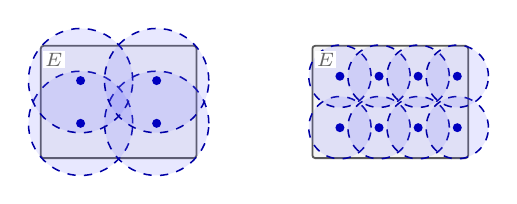
\begin{tikzpicture}[
  scale=0.92,
  every node/.style={font=\scriptsize},
  set/.style={fill=gray!8, draw=black!65, line width=0.65pt},
  ball/.style={fill=blue!55, fill opacity=0.16, draw=blue!65!black, dashed, line width=0.55pt},
  center/.style={circle, fill=blue!75!black, inner sep=1.15pt}
]
  \begin{scope}[shift={(-2.7,0)}]
    \draw[set, rounded corners=1pt] (0,0) rectangle (2.15,1.55);

    \foreach \x/\y in {0.55/0.48,1.60/0.48,0.55/1.07,1.60/1.07} {
      \draw[ball] (\x,\y) circle (0.72);
    }
    \foreach \x/\y in {0.55/0.48,1.60/0.48,0.55/1.07,1.60/1.07} {
      \node[center] at (\x,\y) {};
    }
    \node[black!60, fill=white, inner sep=0.8pt] at (0.18,1.36) {$E$};
  \end{scope}

  \begin{scope}[shift={(1.05,0)}]
    \draw[set, rounded corners=1pt] (0,0) rectangle (2.15,1.55);

    \foreach \x in {0.38,0.92,1.46,2.00} {
      \foreach \y in {0.42,1.13} {
        \draw[ball] (\x,\y) circle (0.43);
      }
    }
    \foreach \x in {0.38,0.92,1.46,2.00} {
      \foreach \y in {0.42,1.13} {
        \node[center] at (\x,\y) {};
      }
    }
    \node[black!60, fill=white, inner sep=0.8pt] at (0.18,1.36) {$E$};
  \end{scope}
\end{tikzpicture}

  \caption{Dots mark a finite $\varepsilon$-net (left) and finer $\delta$-net (right); their balls cover $E$, with $0<\delta<\varepsilon$.}
  \label{fig:total-boundedness-finite-cover}
\end{illustrationfigure}

\begin{theorem} \label{thm:total-bounded-implies-bounded} \hlt{Total Boundedness Implies Boundedness}\\
Let $(X,d)$ be a metric space. If $X$ is totally bounded, then $X$ is bounded.
\begin{proof}
If $X=\emptyset$, it is bounded. Suppose $X\ne\emptyset$, choose finite $1$-net $F\subseteq X$. Then $F\ne\emptyset$; fix $x_0\in F$ and put $R\defeq1+\max\limits_{a\in F}d(a,x_0)$.\\
For $x\in X$, some $a\in F$ satisfies $d(x,a)<1$, so $d(x,x_0)\leq d(x,a)+d(a,x_0)<R$. Hence $X\subseteq B_R(x_0)$.\\
\hlt{Structural Commentary}: A finite unit-ball cover converts finitely many center distances into one radius.\\
\hlt{Key Insight}: One fixed scale already supplies a global bound.
\end{proof}
\end{theorem}

\begin{counterexample} \label{cex:l2-closed-unit-ball-bounded-not-totally-bounded} \hlt{Bounded Need Not Mean Totally Bounded}\\
In $\ell^2(\mathbb{F})$, let $B\defeq\{\mathbf{x}\in\ell^2(\mathbb{F}):\norm{\mathbf{x}}_2\leq1\}$. Then $B\subseteq B_2(0)$, so $B$ is bounded.\\
For the standard unit vectors $(e_n)$, $(\forall\,n\in\N)\,e_n\in B$ and $(\forall\,m\ne n)\,\norm{e_n-e_m}_2=\sqrt{2}$.\\
Any $\frac{1}{2}$-ball contains at most one $e_n$, because two points in such a ball have distance less than $1$.\\
Thus $B$ has no finite $\frac{1}{2}$-net, so $B$ is not totally bounded.
\end{counterexample}

\begin{definition} \label{def:lebesgue-number-open-cover} \hlt{Lebesgue Number}\\
Let $(X,d)$ be a metric space, $\mathcal{U}$ be an open cover of $X$. A number $\delta>0$ is a \hlt{Lebesgue number} for $\mathcal{U}$ iff $(\forall\,x\in X)(\exists\,U\in\mathcal{U})\,B_\delta(x)\subseteq U$.
\end{definition}

\begin{lemma} \label{lem:lebesgue-covering-lemma} \hlt{Lebesgue Covering Lemma}\\
Let $(X,d)$ be a metric space.
\begin{enumerate}[label=(\roman*)]
\setlength{\itemsep}{0pt}
\item If $X$ is sequentially compact, then every open cover of $X$ has a Lebesgue number.
\item If $X$ is compact, then every open cover of $X$ has a Lebesgue number.
\end{enumerate}
\begin{proof}
\begin{enumerate}[label=(\roman*)]
\setlength{\itemsep}{0pt}
\item Let $\mathcal{U}=(U_\alpha)_{\alpha\in A}$ be an open cover of sequentially compact $X$.\\
If $\mathcal{U}$ has no Lebesgue number, choose $(x_n)$ in $X$ satisfying $(\forall\,n\in\N)(\forall\,\alpha\in A)\,B_{\frac{1}{n}}(x_n)\nsubseteq U_\alpha$.\\
Choose a subsequence $x_{n_k}\to x\in X$. Since $\mathcal{U}$ covers $X$, choose $\alpha_0\in A$ and $r>0$ such that $x\in U_{\alpha_0}$ and $B_r(x)\subseteq U_{\alpha_0}$.\\
For sufficiently large $k$, both $d(x_{n_k},x)<\frac{r}{2}$ and $\frac{1}{n_k}<\frac{r}{2}$. If $y\in B_{\frac{1}{n_k}}(x_{n_k})$, then $d(y,x)<r$, so $B_{\frac{1}{n_k}}(x_{n_k})\subseteq U_{\alpha_0}$, a contradiction.
\item If $X$ is compact, then it is sequentially compact by Theorem \ref{thm:compact-sequential-subsequence}. Hence every open cover of $X$ has a Lebesgue number by (i).
\end{enumerate}
\hlt{Structural Commentary}: Bad-radius sequences contradict subsequential convergence; compactness supplies sequential compactness.\\
\hlt{Key Insight}: Near the limit, one cover set absorbs every small ball.
\end{proof}
\end{lemma}

\begin{theorem} \label{thm:compact-complete-totally-bounded} \hlt{Compactness as Complete Finite Resolution}\\
Let $(X,d)$ be a metric space. The following are equivalent:
\begin{enumerate}[label=(\roman*)]
\setlength{\itemsep}{0pt}
\item $X$ is compact;
\item $X$ is complete and totally bounded;
\item $X$ is sequentially compact.
\end{enumerate}
\begin{proof}
\begin{enumerate}[label=(\roman*)]
\setlength{\itemsep}{0pt}
\item[$(i)$]$\Rightarrow (ii)$ Every Cauchy sequence in $X$ converges by Theorem \ref{thm:cauchy-convergence-criterion}(ii), so $X$ is complete. Fix $\varepsilon>0$.\\
Family $\{B_\varepsilon(x):x\in X\}$ is open cover of $X$. By compactness, it has finite subcover, whose centers form a finite $\varepsilon$-net. QED.
\item[$(ii)$]$\Rightarrow (iii)$ Let $(x_n)$ be a sequence in $X$, and put $I_0\defeq\N$ and $n_0\defeq0$.\\
Recursively, suppose $I_{j-1}$ is infinite and choose a finite $\frac{1}{j}$-net $A_j\subseteq X$.\\
If each ball centered in $A_j$ contained $x_n$ for only finitely many $n\in I_{j-1}$, then $I_{j-1}$ would be finite.\\
Hence some $B_{\frac{1}{j}}(a_j)$ contains $x_n$ for infinitely many $n\in I_{j-1}$. Set $I_j\defeq\{n\in I_{j-1}:x_n\in B_{\frac{1}{j}}(a_j)\}$, which is infinite.\\
Choose $n_j\in I_j$ with $n_j>n_{j-1}$. If $k,\ell\geq j$, then $x_{n_k},x_{n_\ell}\in B_{\frac{1}{j}}(a_j)$, so $d(x_{n_k},x_{n_\ell})<\frac{2}{j}$.\\
Given $\varepsilon>0$, choose $J$ with $\frac{2}{J}<\varepsilon$. If $k,\ell\geq J$, then $d(x_{n_k},x_{n_\ell})<\varepsilon$ by the preceding bound.\\
Thus $(x_{n_j})$ is Cauchy and converges in $X$ by completeness.
\item[$(iii)$]$\Rightarrow (i)$ Suppose $X$ is not totally bounded, so some $\varepsilon>0$ admits no finite $\varepsilon$-net.\\
Then $X\ne\emptyset$ as $\emptyset$ is an $\varepsilon$-net for itself. Choose $x_1\in X$, and recursively choose $x_{n+1}\notin\bigcup\limits_{j=1}^{n}B_\varepsilon(x_j)$.\\
Then $(\forall\,j<n)\,d(x_n,x_j)\geq\varepsilon$, so no subsequence is Cauchy.\\
No subsequence converges by Theorem \ref{thm:cauchy-convergence-criterion}(i), contrary to sequential compactness. Thus $X$ is totally bounded.\\
Let $(U_\alpha)_{\alpha\in A}$ be an open cover of $X$. Choose a Lebesgue number $\delta>0$ by Lemma \ref{lem:lebesgue-covering-lemma}(i).\\
Choose a finite $\frac{\delta}{2}$-net $F\subseteq X$. For $z\in F$, choose $\alpha(z)\in A$ with $B_\delta(z)\subseteq U_{\alpha(z)}$.\\
If $x\in X$, then $(\exists\,z\in F)\,x\in B_{\frac{\delta}{2}}(z)\subseteq U_{\alpha(z)}$. Hence the finite family $(U_{\alpha(z)})_{z\in F}$ covers $X$, so $X$ is compact.
\end{enumerate}
\hlt{Structural Commentary}: Finite nets create Cauchy subsequences; Lebesgue numbers convert nets into finite subcovers.\\
\hlt{Key Insight}: Completeness turns finite-resolution control into actual convergence.
\end{proof}
\end{theorem}

Figure \ref{fig:compact-metric-characterization-triangle} summarizes the three equivalent compactness tests.
\begin{illustrationfigure}[H]
  \centering
  \begin{tikzpicture}[
  scale=0.94,
  transform shape,
  >=Stealth,
  every node/.style={font=\scriptsize},
  box/.style={
    draw=blue!60!black,
    fill=blue!5,
    rounded corners=1.5pt,
    align=center,
    inner xsep=4pt,
    inner ysep=3pt,
    minimum width=2.75cm,
    minimum height=0.58cm
  },
  arrow/.style={<->, line width=0.65pt, black!70}
]
  \node[box] (compact) at (0,0.95)
    {$\begin{array}{c}
      X\ \mathrm{compact}\\[-1pt]
      \mathcal{U}\Rightarrow\mathcal{U}_0,\ |\mathcal{U}_0|<\infty
    \end{array}$};
  \node[box, minimum width=3.35cm] (finite) at (-2.25,-0.70)
    {$\begin{array}{c}
      X\ \mathrm{complete+t.b.}\\[-1pt]
      X\subseteq B_\varepsilon(F_\varepsilon),\ |F_\varepsilon|<\infty
    \end{array}$};
  \node[box, minimum width=3.00cm] (seq) at (2.25,-0.70)
    {$\begin{array}{c}
      X\ \mathrm{seq.\ compact}\\[-1pt]
      x_n\Rightarrow x_{n_k}\to x\in X
    \end{array}$};

  \draw[arrow] (compact) -- (finite);
  \draw[arrow] (finite) -- (seq);
  \draw[arrow] (seq) -- (compact);
\end{tikzpicture}

  \caption{The proof cycle connects finite subcovers, completeness with finite $\varepsilon$-nets, and convergent subsequences.}
  \label{fig:compact-metric-characterization-triangle}
\end{illustrationfigure}

\begin{proposition} \label{prop:compact-metric-spaces-separable} \hlt{Compact Metric Spaces Are Separable}\\
Let $(X,d)$ be a compact metric space. Then $X$ contains an at most countable set $D$ such that $\overline{D}^{\,X}=X$.
\begin{proof}
The space $X$ is totally bounded by Theorem \ref{thm:compact-complete-totally-bounded}, direction $(i)\Rightarrow(ii)$.\\
Choose finite $\frac{1}{n}$-nets $F_n\subseteq X$ for $n\in\N$. Set $D\defeq\bigcup\limits_{n=1}^{\infty}F_n$. The set $D$ is at most countable by Corollary \ref{cor:at-most-countable-union-at-most-countable}.\\
Let $x\in X$ and $r>0$, and choose $n\in\N$ with $\frac{1}{n}<r$. Some $a\in F_n$ satisfies $d(x,a)<\frac{1}{n}<r$, so $a\in B_r(x)\cap D$.\\
Thus every open ball centered at $x$ meets $D$, so $x\in\overline{D}^{\,X}$. Therefore $\overline{D}^{\,X}=X$, and $X$ is separable.\\
\hlt{Structural Commentary}: Finite nets at reciprocal scales form an at most countable dense union.\\
\hlt{Key Insight}: One sufficiently fine net meets every prescribed ball.
\end{proof}
\end{proposition}
